\documentclass[9pt]{beamer}
\usetheme{CambridgeUS}
\usepackage[T1]{fontenc}
\usefonttheme{serif}
\usepackage[utf8]{inputenc}
% \usepackage{xeCJK}
\usepackage{xcolor}


\usepackage{amsmath,amsfonts,amsthm,amssymb,commath}
\usepackage{comment}
\usepackage{natbib}
\usepackage{hyperref}
\usepackage{graphicx,float,wrapfig}
\usepackage{mathtools}
\usepackage{esint}
\usecolortheme{dolphin}
\usepackage{bm}
\usepackage{centernot}
\usepackage[]{algorithm2e}

\DeclareMathOperator*{\argmax}{arg\,max}
\DeclareMathOperator*{\argmin}{arg\,min}

\DeclareMathOperator{\imag}{Im}
\DeclareMathOperator{\real}{Re}
\DeclareMathOperator{\Arg}{Arg}
\DeclareMathOperator{\Arctan}{Arctan}
\DeclareMathOperator{\degree}{degree}
\DeclareMathOperator{\ind}{ind}
\DeclareMathOperator{\dist}{dist}
\DeclareMathOperator{\Log}{Log}
\DeclareMathOperator{\Res}{Res}
\DeclareMathOperator{\var}{var}
\DeclareMathOperator{\Id}{Id}
\DeclareMathOperator{\CVX}{CVX}
\DeclareMathOperator{\Dom}{Dom}
\DeclareMathOperator{\inter}{Int}

\newcommand{\kl}[1]{\mathcal{D}_{\text{KL}}(#1)}
\newcommand{\E}{\mathbb{E}}

%\beamerdefaultoverlayspecification{<
\newcommand{\R}{\mathbb{R}}
\newcommand{\N}{\mathbb{N}}
\newcommand{\cB}{\mathcal{B}}
\newcommand{\cP}{\mathcal{P}}
\newcommand{\Cov}{\text{Cov}}
\newcommand{\Var}{\text{Var}}
\newcommand{\bbar}[1]{\bar{\bar{#1}}}
\newcommand{\of}[1]{\left(#1\right)}
\newcommand{\off}[1]{\left[#1\right]}
\newcommand{\offf}[1]{\left\{#1\right\}}
%\newcommand{\norm}[1]{\left\|#1\right\|}
\newcommand{\hl}[1]{\textbf{\textcolor{myNewColorA}{#1}}}
\newcommand{\bx}{\mathbf{x}}
\newcommand{\supp}{\text{\textbf{supp} }}
\newcommand{\cN}{\mathcal{N}}
\newcommand{\cC}{\mathcal{C}}

% set colors
\definecolor{myNewColorA}{RGB}{51,0,111}
\definecolor{myNewColorB}{RGB}{232,211,162}
\definecolor{myNewColorC}{RGB}{145,123,76}
\setbeamercolor*{palette primary}{bg=myNewColorC}
\setbeamercolor*{palette secondary}{bg=myNewColorB, fg = white}
\setbeamercolor*{palette tertiary}{bg=myNewColorA, fg = white}
\setbeamercolor*{titlelike}{fg=myNewColorA}
\setbeamercolor*{title}{bg=myNewColorA, fg = white}
\setbeamercolor*{item}{fg=myNewColorA}
\setbeamercolor*{caption name}{fg=myNewColorA}
\usefonttheme{professionalfonts}

%------------------------------------------------------------
\titlegraphic{
\includegraphics[height=2.5cm]{uw logo.png}}

\setbeamerfont{title}{size=\large}
\setbeamerfont{subtitle}{size=\small}
\setbeamerfont{author}{size=\small}
\setbeamerfont{date}{size=\small}
\setbeamerfont{institute}{size=\small}
\setbeamertemplate{itemize item}[circle]
\setbeamertemplate{itemize subitem}[default]
\title[University of Washington]{Graphical Semi-Supervised Learning}
\subtitle{AMATH 563}
\author[]{Lucas Cassin Cruz Burke}




%------------------------------------------------------------
%This block of commands puts the table of contents at the 
%beginning of each section and highlights the current section:
%\AtBeginSection[]
%{
%  \begin{frame}
%    \frametitle{Contents}
%    \tableofcontents[currentsection]
%  \end{frame}
%}
\AtBeginSection[]{
  \begin{frame}
  \vfill
  \centering
  \begin{beamercolorbox}[sep=8pt,center,shadow=true,rounded=true]{title}
    \usebeamerfont{title}\insertsectionhead\par%
  \end{beamercolorbox}
 \vfill
  \end{frame}
}
%------------------------------------------------------------

\begin{document}

%The next statement creates the title page.
\frame{\titlepage}
%------------------------------------------------------------
% Introduction: Semi-Supervised Learning

\begin{frame}{Semi Supervised Learning}
    \begin{itemize}
        \item Semi-supervised learning is the problem of predicting the labels of an unlabeled set of data $(x_i, y_i)_{i=M+1}^N$ based on a subset of labeled datapoints $(x_i, y_i)_{i=1}^M$. 
        \item Graphical SSL algorithms build a graph on top of the $x_i$'s and formulate the problem as a regularized regression problem on $G$ using the Graph Laplacian matrix, which can be used to learn the structure of the underlying manifold.
    \end{itemize}
    \begin{figure}[h!]
      \centering
      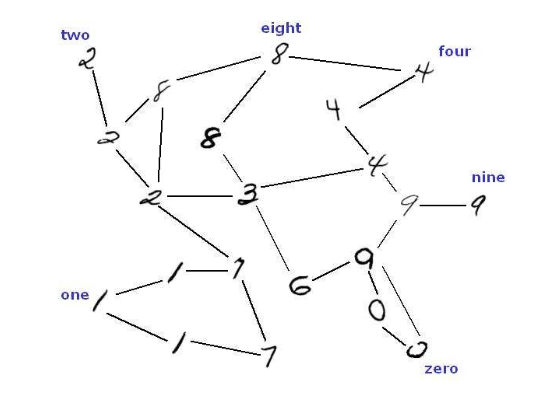
\includegraphics[width=5cm]{digitSSL_ex.png} % Replace with the actual file name and extension
    \end{figure}
\end{frame}

%------------------------------------------------------------
% Probit model

\begin{frame}{Probit model \& Laplacian based regularization}
    \begin{itemize}
      \item We assume our generating process is of the form $y_j = \operatorname{sign} (f(\mathbf x_j) + \varepsilon_j)$ with normally distributed noise $\varepsilon_j \sim \psi$.
      \item We then formulate a binary classification task in the RKHS framework using the Probit loss function and the regularization function given by
      $$\mathbf f^* = \argmin_{f \in \mathbb R^M} \left\{ - \sum_{j=1}^N \log \Psi (f_j y_j) + \beta \mathbf f^T C \mathbf f \right\}$$where $C = \left( \Delta + \tau^2 I \right)^{-\alpha/2}$ and $\Delta = D - W$ is the graph Laplacian.
      \item $C$ is strictly PDS and defines an RKHS, hence by the reproducing property we have $$\mathbf f^* = C(:, 1:N)C(1:N, 1:N)^{-1}\mathbf z^*$$ where $\mathbf z^* = \argmin_{\mathbf z \in \mathbb R^N} \left\{-\sum_{j=1}^N \log \Psi (y_j z_j) + \beta \mathbf z^T C(1:N, 1:N)^{-1} \mathbf z \right\}$.
    \end{itemize}
  
\end{frame}

%------------------------------------------------------------
% A related problem

\begin{frame}{A related problem}
  Let us briefly ponder the related inhomogeneous differential equation $$C \mathbf f = \left( \Delta + \tau^2 I \right)^{-\alpha/2} \mathbf f= \mathbf h$$
  \begin{itemize}
    \item $C$ is linear and elliptic, and so the solution can be written using the Green's function $G$ as $$\mathbf f(\mathbf x) = \int h(\mathbf z) G(\mathbf x, \mathbf z) d \mathbf z$$ where $(CG)(\mathbf x, \mathbf z) = \delta(\mathbf x - \mathbf z)$.
    \item It turns out that this Green's function is given by the Matérn kernel functional $$C_\nu (d) = \sigma^2 \frac{2^{1-\nu}}{\Gamma(\nu)}\left( \sqrt{2\nu} \frac{d}{\rho} \right)^\nu K_\nu \left( \sqrt{2 \nu} \frac{d}{\rho}\right)$$
    \item The Matérn family includes the exponential kernel ($C_{1/2}$) and the Gaussian kernel ($C_\infty$) as particular cases. 
  \end{itemize}
\end{frame}

%------------------------------------------------------------
% Probit model

\begin{frame}{SSL by diffusion: Laplace \& Poisson methods}
  \begin{itemize}
    \item \textbf{Laplace method}: Treat labeled points as Dirichlet boundary conditions. 
    \begin{figure}[h!]
      \centering
      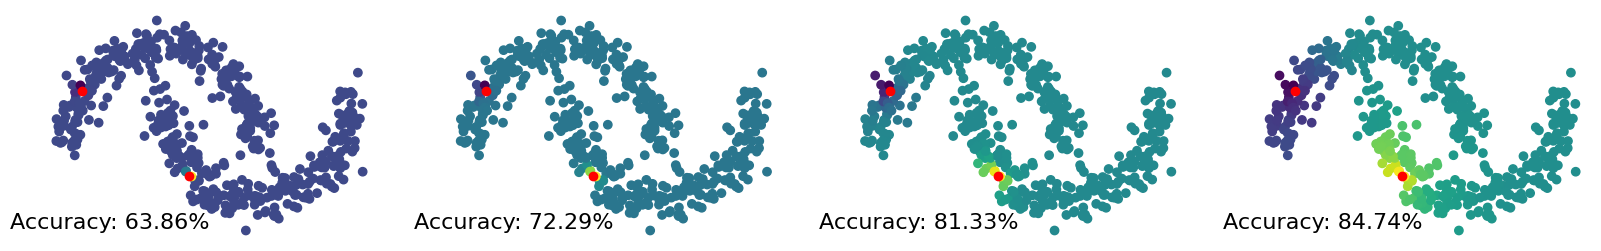
\includegraphics[width=11cm]{LaplaceSSL.png} % Replace with the actual file name and extension
      \caption{Heat diffusion with Dirichlet boundary conditions at labeled points.}
    \end{figure}
    \item \textbf{Poisson method}: Treat labeled points as heat sources/sinks.
    \begin{figure}[h!]
      \centering
      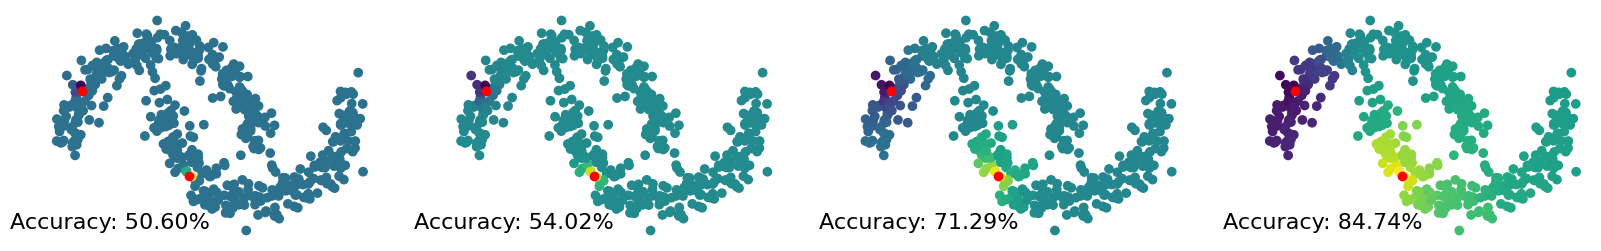
\includegraphics[width=11cm]{PoissonSSL.png} % Replace with the actual file name and extension
      \caption{Heat diffusion with sources/sinks at labeled points.}
    \end{figure}
  \end{itemize}
  \small{\textit{KNN (K=5). Gaussian kernel. Time steps incrementing by powers of 10 from $10^2$ to $10^5$.}}
\end{frame}

%------------------------------------------------------------
% Probit model

\begin{frame}{Matérn kernel parameters}
  \begin{figure}[h!]
    \centering
    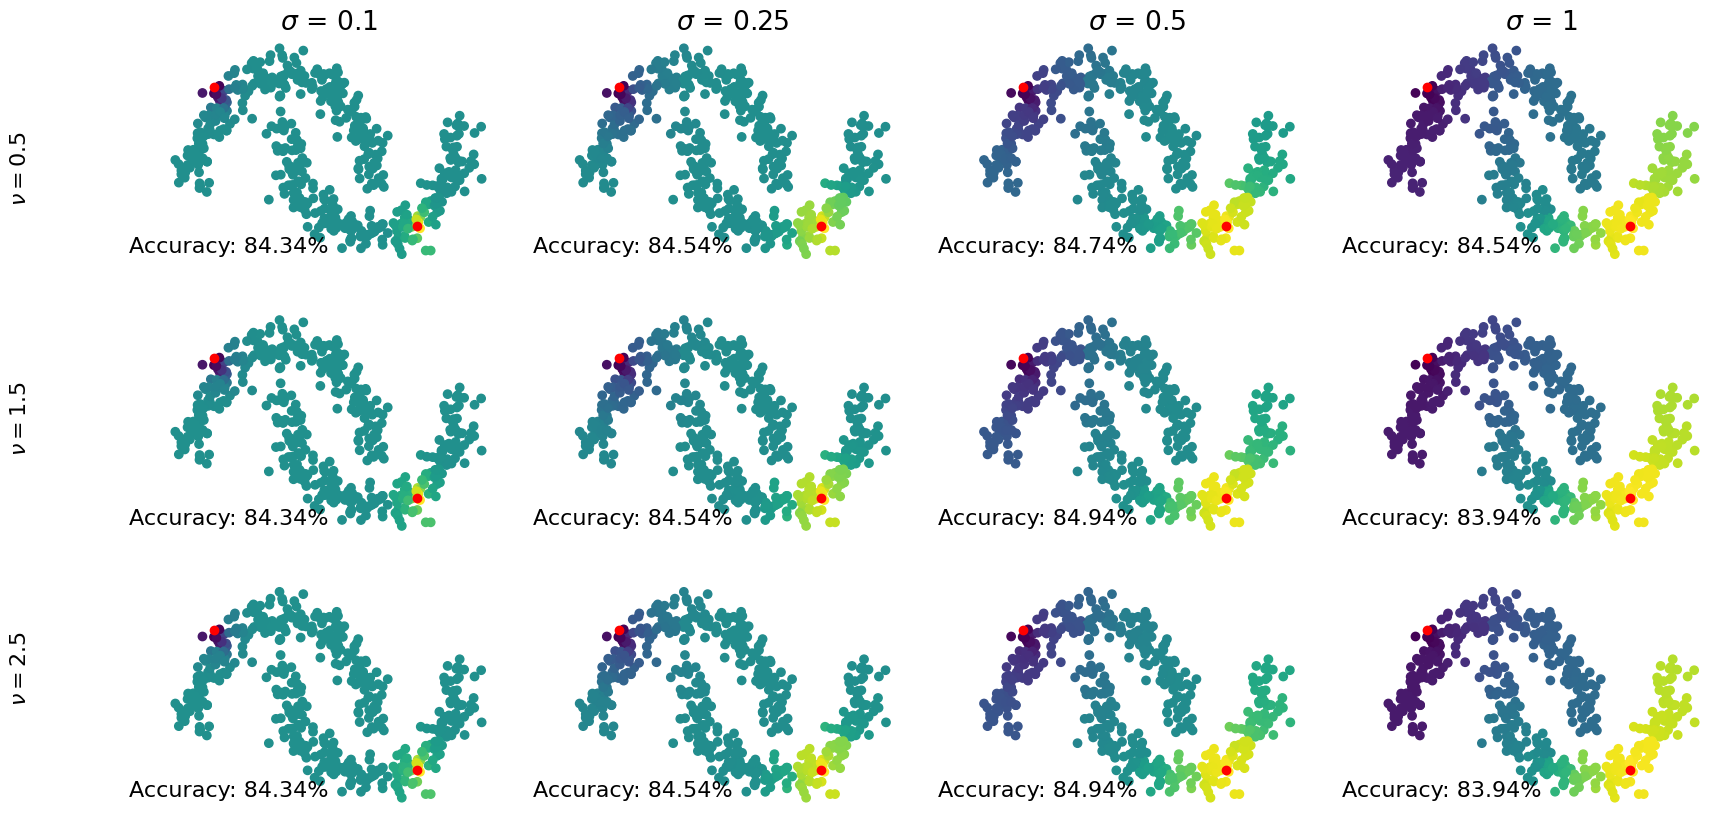
\includegraphics[width=11cm]{laplace_cv.png} % Replace with the actual file name and extension
    \caption{Laplace method solve for different values of $\nu$ and $\sigma$.}
  \end{figure}
\end{frame}

%------------------------------------------------------------

\begin{frame}{Comparing Graphical SSL methods}
  
\begin{figure}[h!]
  \centering
  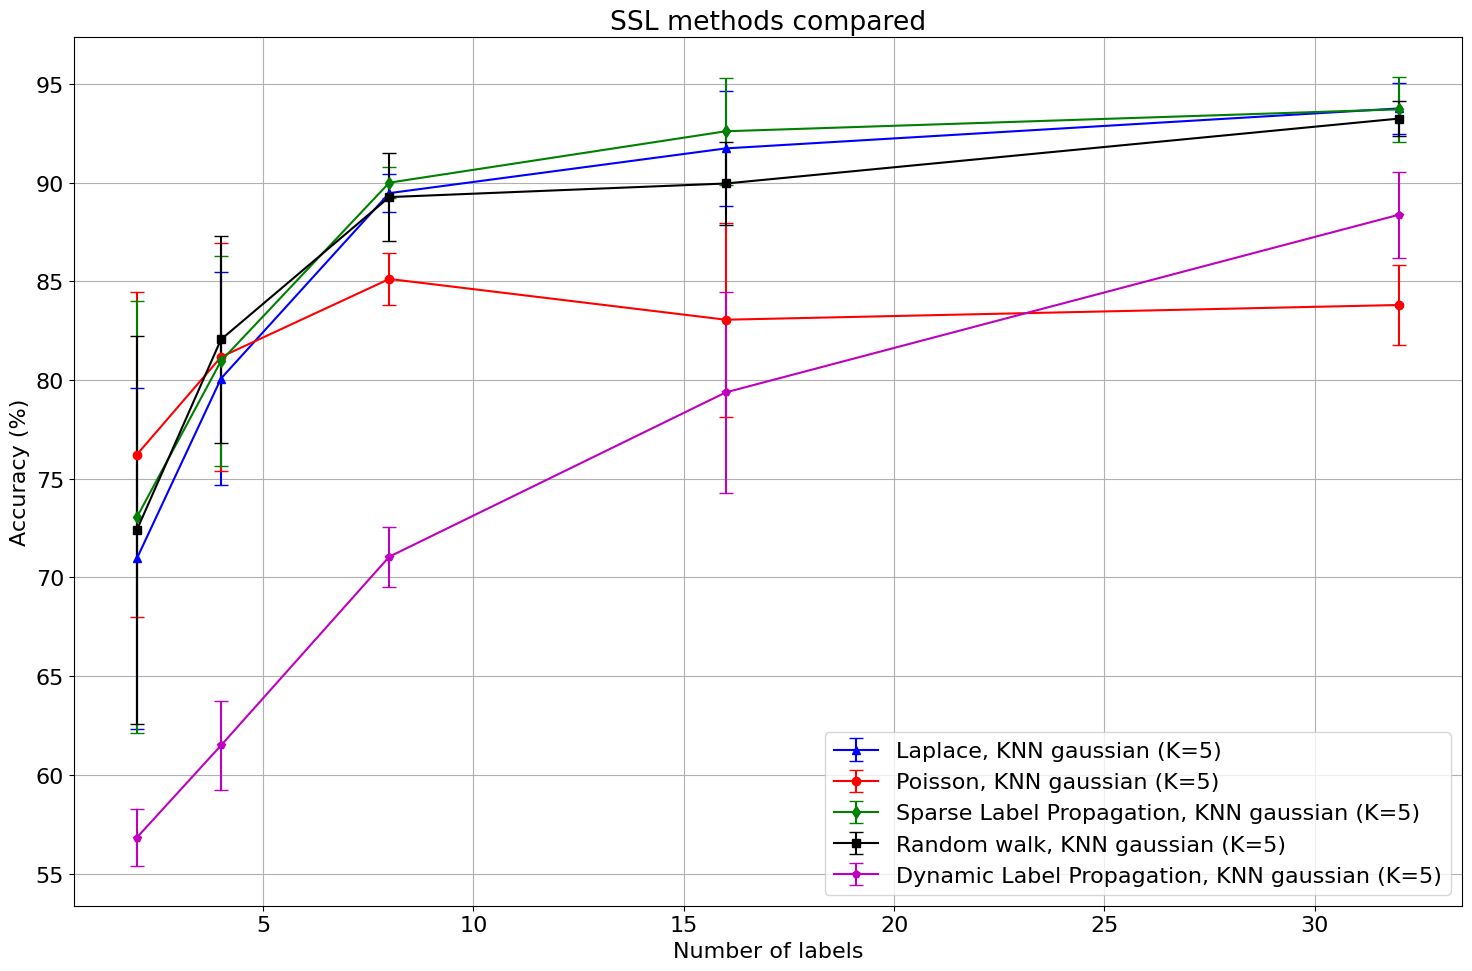
\includegraphics[width=10cm]{ssl_methods_comp.png} % Replace with the actual file name and extension
  \caption{Comparison of graphical SSL method performance on Two Moons Probit problem.}
\end{figure}

\end{frame}

%------------------------------------------------------------

\section{Thank you :)}

%------------------------------------------------------------
% Probit

% References
\begin{frame}{References}
  \begin{enumerate}
    \item Mikhail Belkin and Partha Niyogi. Semi-supervised learning on riemannian manifolds. \textit{Machine learning}, 56:209–239, 2004.
    \item Viacheslav Borovitskiy, Iskander Azangulov, Alexander Terenin, Peter Mostowsky, Marc Deisenroth, and Nicolas Durrande. Matérn gaussian processes on graphs. In \textit{International Conference on Artificial Intelligence and Statistics}, pages 2593–2601. PMLR, 2021.
    \item Franca Hoffmann, Bamdad Hosseini, Zhi Ren, and Andrew M Stuart. Consistency of semi-supervised learning algorithms on graphs: Probit and one-hot methods. \textit{The Journal of Machine Learning Research}, 21(1):7549–7603, 2020.
    \item Daniel Sanz-Alonso and Ruiyi Yang. The spde approach to matérn fields: Graph representations. \textit{Statistical Science}, 37(4):519–540, 2022.
    \item Xiaojin Jerry Zhu. Semi-supervised learning literature survey. 2005.
    \item Jeff Calder. GraphLearning Python Package. Zenodo. 2022.
    \item 
  \end{enumerate}
\end{frame}


\end{document}